\begin{naloga}{Sergio Cabello}{Teorija OR 5.9.2017}
\begin{vprasanje}
Obravnavamo manjši sudoku velikosti $4\times 4$ s slike~\fig.
Vanj vpisujemo števila med $1$ in $4$.
Vsako število se pojavi natanko enkrat v vsaki vrstici,
vsakem stolpcu in vsakem od $4$ kvadratov velikosti $2 \times 2$,
omejenih z debelejšo črto.
Opiši celoštevilski linearni program za reševanje takega problema
oz.~za določanje, da rešitev ne obstaja.
Koliko spremenljvk in pogojev ima linearni program?

\begin{slika}
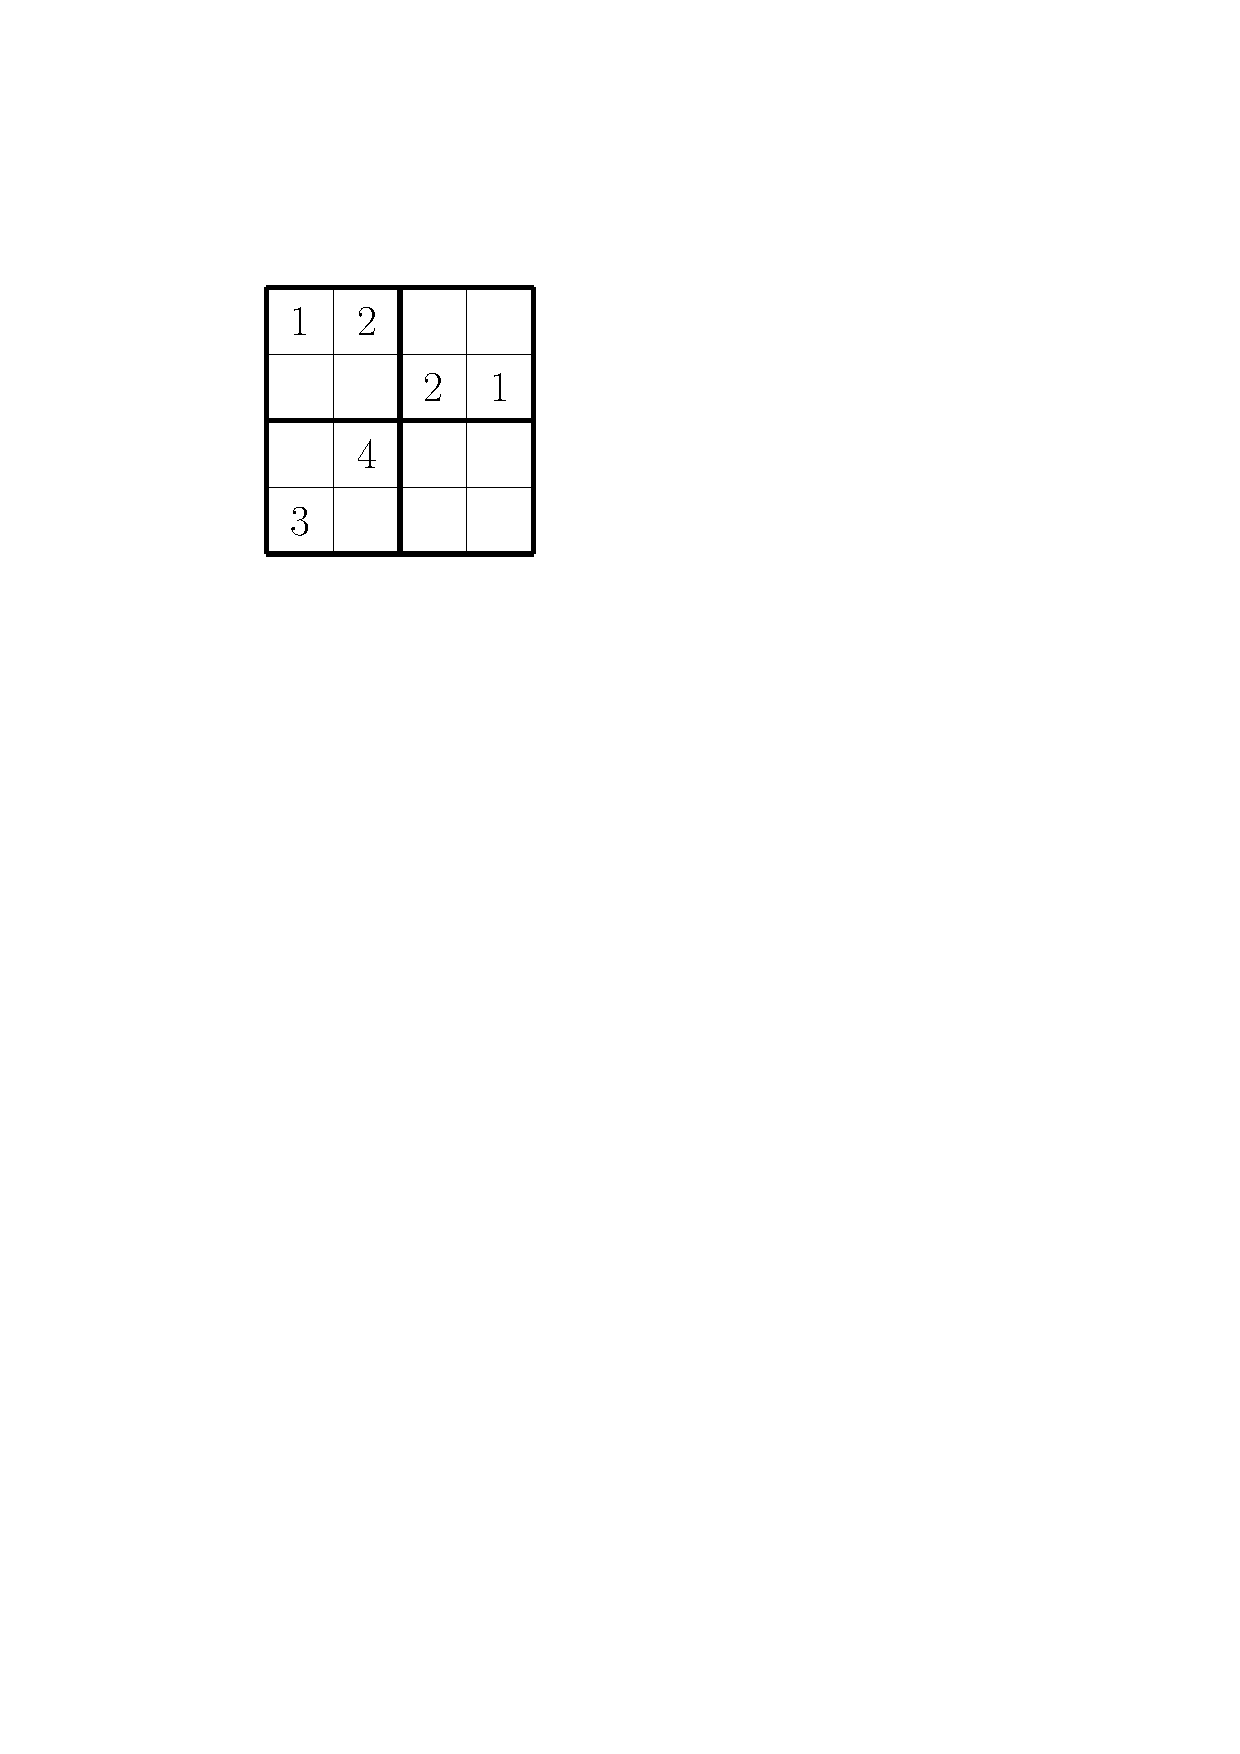
\includegraphics[scale=.7]{slike/sudoku}
\podnaslov{Primer sudokuja}
\end{slika}
\end{vprasanje}

\begin{odgovor}
Za $i, j, k \in \{1, 2, 3, 4\}$ bomo uvedli spremenljivko $x_{ijk}$,
katere vrednost interpretiramo kot
$$
x_{hij} = \begin{cases}
1; & \text{na polje $(i, j)$ vpišemo število $k$, in} \\
0  & \text{sicer.}
\end{cases}
$$
Zapišimo omejitve za celoštevilski linearni program.
Zanima nas samo njegova dopustnost, tako da ciljna funkcija ni pomembna.
\begin{alignat*}{2}
\forall i, j, k \in \{1, 2, 3, 4\}: &\ &
0 \le x_{ijk} &\le 1, \quad x_{ijk} \in \Z
\opis{V vsako polje vpišemo eno število}
\forall i, j \in \{1, 2, 3, 4\}: &\ & \sum_{k=1}^4 x_{ijk} &= 1
\opis{Vsako število se pojavi enkrat v vsaki vrstici in stolpcu}
\forall i, k \in \{1, 2, 3, 4\}: &\ & \sum_{j=1}^4 x_{ijk} &= 1 \\
\forall j, k \in \{1, 2, 3, 4\}: &\ & \sum_{i=1}^4 x_{ijk} &= 1
\opis{Vsako število se pojavi enkrat v vsakem kvadratku $2 \times 2$}
\forall i, j \in \{0, 2\} \ \forall k \in \{1, 2, 3, 4\}: &\ &
\sum_{i'=1}^2 \sum_{j'=1}^2 x_{i+i',j+j',k} &= 1
\opis{Že vpisana števila}
x_{111} = x_{122} = x_{232} &=& x_{241} = x_{324} = x_{413} &= 1
\end{alignat*}
Opisani celoštevilski linearni program
ima $4^3 = 64$ celoštevilskih spremenljivk
in $2 \cdot 4^3 + 4 \cdot 4^2 + 6 = 198$ pogojev.
\end{odgovor}
\end{naloga}
